\documentclass[problem]{mcs}

\newcommand{\neutr}{\ensuremath{\mathbf{N}}}

\begin{pcomments}
  \pcomment{MQ_3color_XOR}
  \pcomment{variant of CP_3color_OR_gate, PS_3color_SAT}
  \pcomment{ARM Mar 22, 2014}
\end{pcomments}

\pkeywords{
coloring
xor
}

%%%%%%%%%%%%%%%%%%%%%%%%%%%%%%%%%%%%%%%%%%%%%%%%%%%%%%%%%%%%%%%%%%%%%
% Problem starts here
%%%%%%%%%%%%%%%%%%%%%%%%%%%%%%%%%%%%%%%%%%%%%%%%%%%%%%%%%%%%%%%%%%%%%
\begin{problem}
Consider the graph in Figure~\ref{fig:3color-XOR}.  We designate the
vertices connected in the triangle on the left as
\emph{color-vertices}; since they form a triangle, they are forced to
have different colors in any coloring of the graph.  The colors
assigned to the color-vertices will be called $\true, \false$ and
$\neutr$.  The dotted lines indicate edges to the color-vertex
$\neutr$.

\bparts

\ppart Prove that, in any valid 3-coloring of the graph, neither $P$ nor
$Q$ are colored $\neutr$.

\begin{solution}
If there is a valid 3-coloring (or more generally, any valid coloring)
then the dotted edges ensure that $P$ and $Q$ are not colored as
$\neutr$ in that coloring.
\end{solution}

\examspace[2cm]

\ppart Prove that, for any coloring of just $P$ and $Q$ where neither
is colored $\neutr$, we can extend that coloring to a 3-coloring
for the whole graph, and in any 3-coloring the vertex
labeled $P \QXOR Q$ is colored with the $\QXOR$ of the colors of
vertices $P$ and $Q$.

\begin{solution}
If neither $P$ nor $Q$ are colored $\neutr$, then both $P$ and $Q$
have to be colored $\true$ or $\false$.

There are two cases to consider.

\inductioncase{Case 1}: $P$ and $Q$ have different truth-colors.

Then the vertex adjacent to $P$ and $Q$ must be colored $\neutr$, the
vertex it above must be colored $\false$, and hence the vertex
labelled $(P \QXOR Q)$ is colored $\true$, as required.

Moreover, the rest of the graph can be 3-colored.  To show this, let's
call the vertex adjacent to $P$ and the $\neutr$-vertex the
``$\bar{P}$'' vertex, since it must be colored with the negation of the
$P$ color.  Hence in this case, the $\bar{P}$-vertex and $Q$ have the
same color.  This allows the vertex adjacent to $Q$ and the
$\bar{P}$-vertex to be colored with the $P$ color and the vertex above
it to be colored $\neutr$, which is consistent with the $(P \QXOR
Q)$-vertex coloring.

\inductioncase{Case 2}: $P$ and $Q$ have the same truth-color.

In this case, the $\bar{P}$-vertex and $Q$ have different colors.  Now
the same argument for Case 1 can be repeated to conclude that the
$(P \QXOR Q)$-vertex must be colored $\false$.

\end{solution}

\eparts

\end{problem}

\begin{figure}\inbook{[h]}
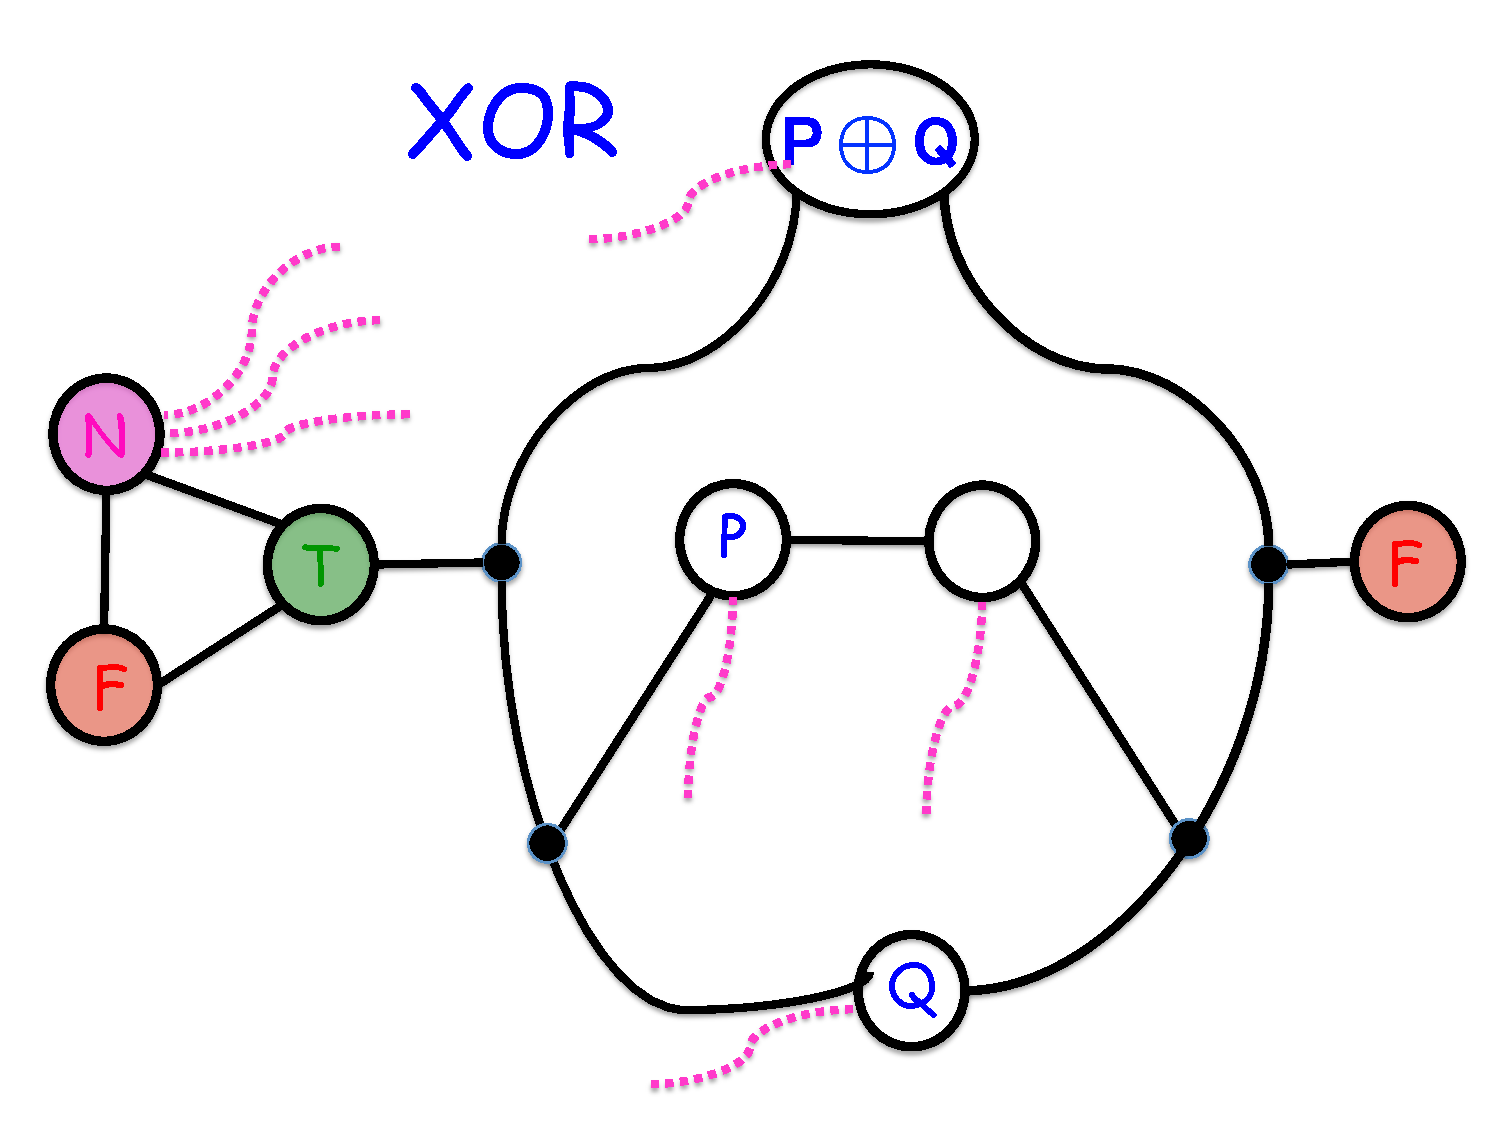
\includegraphics[width=4in]{3color-XOR}
\caption{A 3-color $\QXOR$-gate}
\label{fig:3color-XOR}
\end{figure}

%%%%%%%%%%%%%%%%%%%%%%%%%%%%%%%%%%%%%%%%%%%%%%%%%%%%%%%%%%%%%%%%%%%%%
% Problem ends here
%%%%%%%%%%%%%%%%%%%%%%%%%%%%%%%%%%%%%%%%%%%%%%%%%%%%%%%%%%%%%%%%%%%%%

\endinput
